\subsubsection{Listar}

  \paragraph{}Para mostrar esta lista, es necesario establecer el asesor para
  el que mostrar las reuniones disponibles. Para ello, habrá que elegir
  el asesor en la lista desplegable que se muestra en la figura
  \ref{capturaPantallaSelectAsesor}.

  \paragraph{}También habrá que seleccionar el curso académico para el que
  listar las reuniones del asesor seleccionado. La figura
  \ref{capturaPantallaSelectAsesorCursoAcademico} muestra una captura de
  pantalla de la lista desplegable para seleccionarlo.

  \paragraph{}Por último, habrá que elegir el alumno para el que mostrar las
  reuniones existentes. Para ello, se seleccionará en una lista desplegable,
  tal y como muestra la captura de pantalla de la figura
  \ref{capturaPantallaSelectAlumno}.

  \begin{figure}[!ht]
    \begin{center}
      \fbox{
      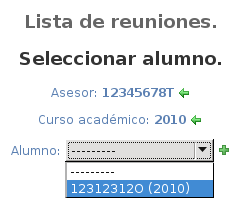
\includegraphics[scale=0.55]{4.Funcionamiento_Aplicacion/4.3.Gestion/4.3.1.Administrador_Principal/4.3.1.15.Reunion/select_alumno.png}
      }
      \caption{Captura de pantalla de los enlaces para seleccionar listado de alumnos para el usuario \textit{Administrador principal}.}
      \label{capturaPantallaSelectAlumno}
    \end{center}
  \end{figure}

  \paragraph{}Nótese que si no existieran elementos disponibles en el sistema,
  la lista desplegable aparecería vacía. Por tanto, se proporciona al usuario
  un icono, representado por una cruz verde, para añadir nuevos elementos al
  sistema. Este icono es el mostrado en la figura \ref{capturaBotonAdd}. Al
  pulsar dicho botón, aparecerá la ventana de creación de un nuevo elemento.

  \paragraph{}Una vez seleccionado el asesor entre los disponibles, se muestra
  la lista completa de reuniones que aparecen en el sistema. La figura
  \ref{capturaPantallaListaReunionesAdminPrincipal} muestra una captura de
  pantalla de la lista de reuniones.

  \begin{figure}[!ht]
    \begin{center}
      \fbox{
      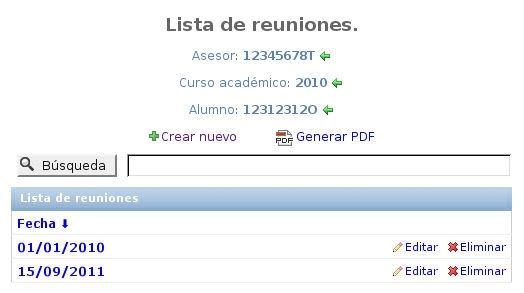
\includegraphics[scale=0.55]{4.Funcionamiento_Aplicacion/4.3.Gestion/4.3.1.Administrador_Principal/4.3.1.15.Reunion/lista_reuniones.png}
      }
      \caption{Captura de pantalla de la lista de reuniones para el usuario \textit{Administrador principal}.}
      \label{capturaPantallaListaReunionesAdminPrincipal}
    \end{center}
  \end{figure}
